\section{Discussion and Evaluations}  \label{sec:discussion_evaluations}

In this section, VeTrac performance is compared with three state of the art schemes, namely \ac{lpr} scheme \cite{simonyan2014very}, \ac{re-id} scheme \cite{liu2017provid} and \ac{hris} scheme \cite{zheng2012reducing}.
The data used in the evaluation contains of 7,206,500 snapshots from more than 1000 cameras in the road network in one of China's big cities during a specific day from 8 AM to 5 PM.
Furthermore, to conduct the study, they used on a server with Intel Xeon E5-2682 processor that has 2.50 GHz.
In addition, the server has 32 GB Video RAM as it is equiped with NVIDIA RTX 2080Ti graphics card.
The data collected was used to train the \ac{mds} block.
It took VeTrac around 3 hours to reconstruct vehicle trajectories from almost one million snapshots and almost 16 hours to process the whole data.
As shown in \Cref{fig:performance-comparison}, VeTrac performance outweigh the performance of all state-of-the-art solutions in the city, and inside city, as presented in \Cref{fig:performance-comparison-city}, with at least 40\% in accuracy (acc), precision (p), and recall (r).

\begin{figure}
\centering
  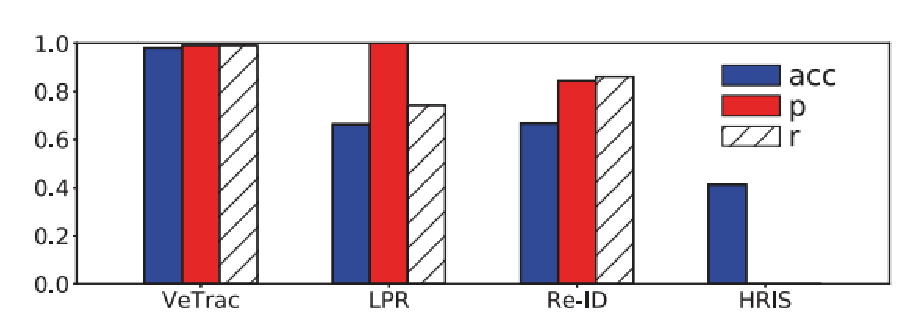
\includegraphics[width=0.9\linewidth]{figures/performance-comparison.eps}
  \caption{Performance comparison in express way \cite{tong2021large}}
  \label{fig:performance-comparison}
  %\vspace{-5mm}
\end{figure}

\begin{figure}
\centering
  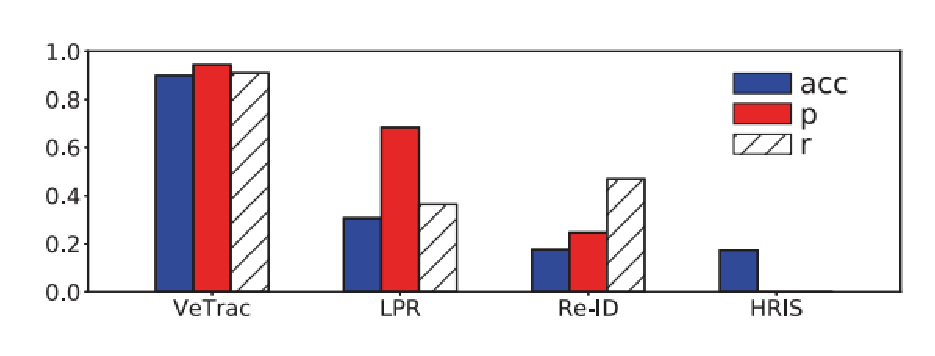
\includegraphics[width=0.9\linewidth]{figures/performance-comparison-urban.eps}
  \caption{Performance comparison inside city \cite{tong2021large}}
  \label{fig:performance-comparison-city}
  %\vspace{-5mm}
\end{figure}

Comparing the performance of VeTrac with the state-of-the-art networks for the blue ground-truth bus route in the city, depicted in \Cref{fig:bus-route-reconsturction-comparison}(a), the output is shown in \Cref{fig:bus-route-reconsturction-comparison}(b).
It is crystal clear that VeTrac reconstructed the correct track of the bus route with almost 100\% accuracy, while the routes generated in \ac{lpr}, \ac{re-id}, and \ac{hris} have lots of deficiencies.

\begin{figure*}
\centering
  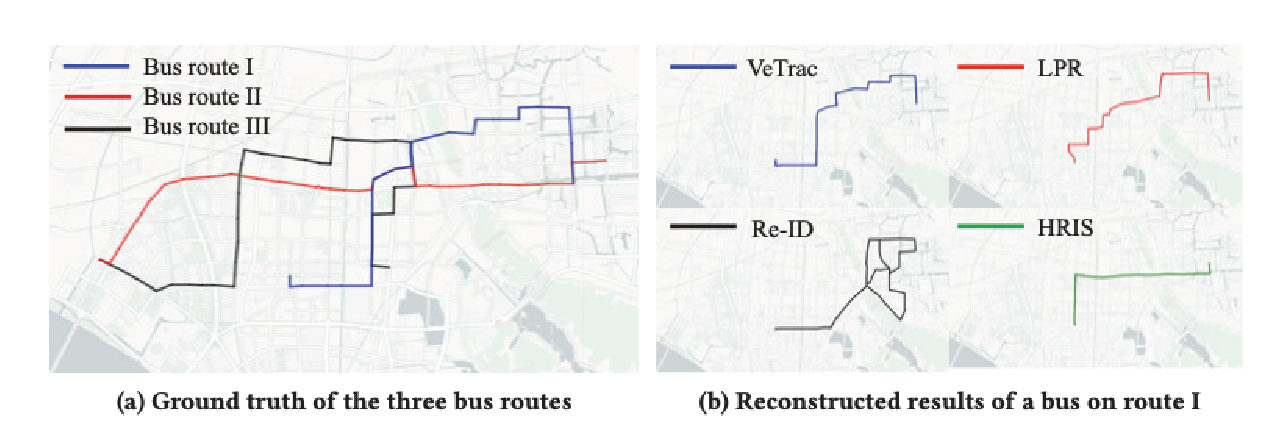
\includegraphics[width=0.9\linewidth]{figures/bus-route-reconstruction-comparison.eps}
  \caption{Bus route reconstruction comparison \cite{tong2021large}}
  \label{fig:bus-route-reconsturction-comparison}
  %\vspace{-5mm}
\end{figure*}
